\section{Results}
\label{sec:result}
\subsection{RQ1. Change patterns}
\label{sec:result:pattern}


%The taxonomy includes change of lock type, change of lock variable, synchronization addition, synchronization removal, lock release, volatile addition, volatile removal, class replacement, thread-safe class replacement, thread management, thread status management,

\begin{table*}
\zhong{Please delete this table.}
	\centering
	\caption{Taxonomy}
	\begin{tabular}{|c|c|c|}\hline
		Type&Example&Occurrence\\\hline
		Changing lock type&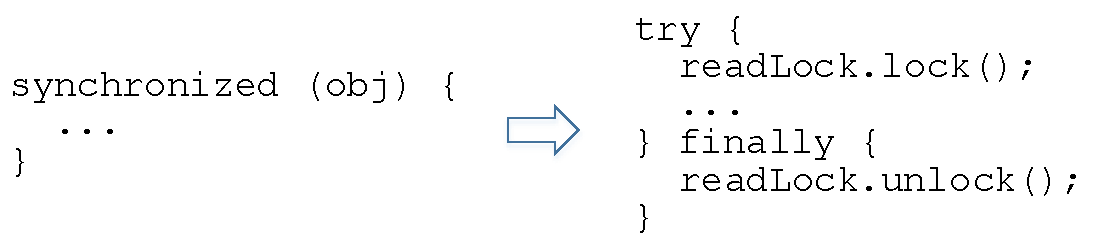
\includegraphics[scale=0.35]{pattern1}&4\\\hline
		Changing lock instance&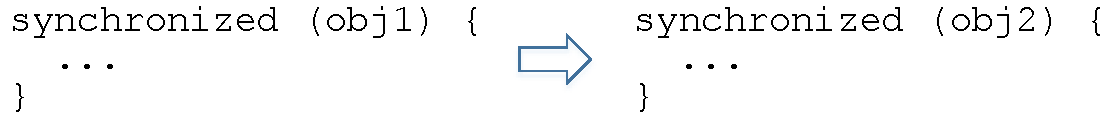
\includegraphics[scale=0.35]{pattern2}&6\\\hline
		Changing critical section&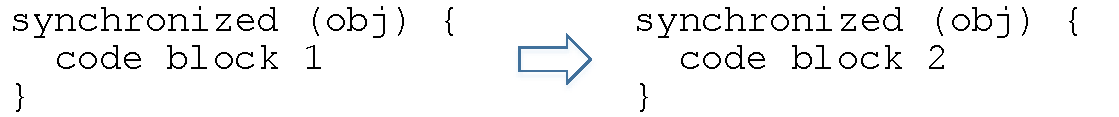
\includegraphics[scale=0.35]{pattern3}&35\\\hline
		Adding or removing \texttt{volatile}&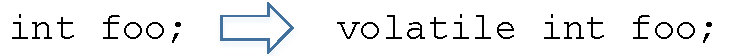
\includegraphics[scale=0.35]{pattern4}&47\\\hline
		Thread-safe class replacement&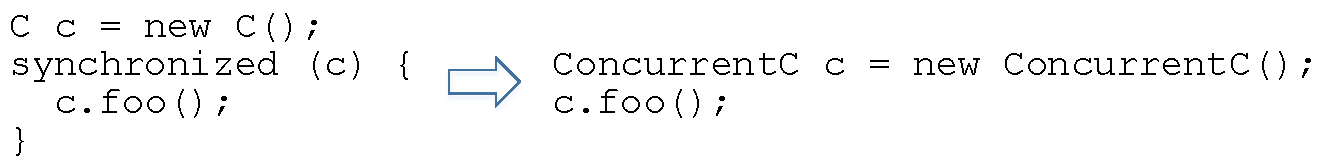
\includegraphics[scale=0.35]{pattern5}&32\\\hline
		Thread management&&\\\hline
		%Other class replacement&Some other concurrent related class replacement&\\\hline
	\end{tabular}
\end{table*}

%Switch to another type of lock
%Switch to another lock instace
%Change critical sections, which are protected by synchronization
%Add or remove 'volatile' modifier of a class field
%Use thread-safe class instead of handling concurrency control manually

Table~\ref{} and \ref{} show an overview of our extracted change patterns. \zhong{Please explain the columns.}

\begin{figure*}
	\centering
	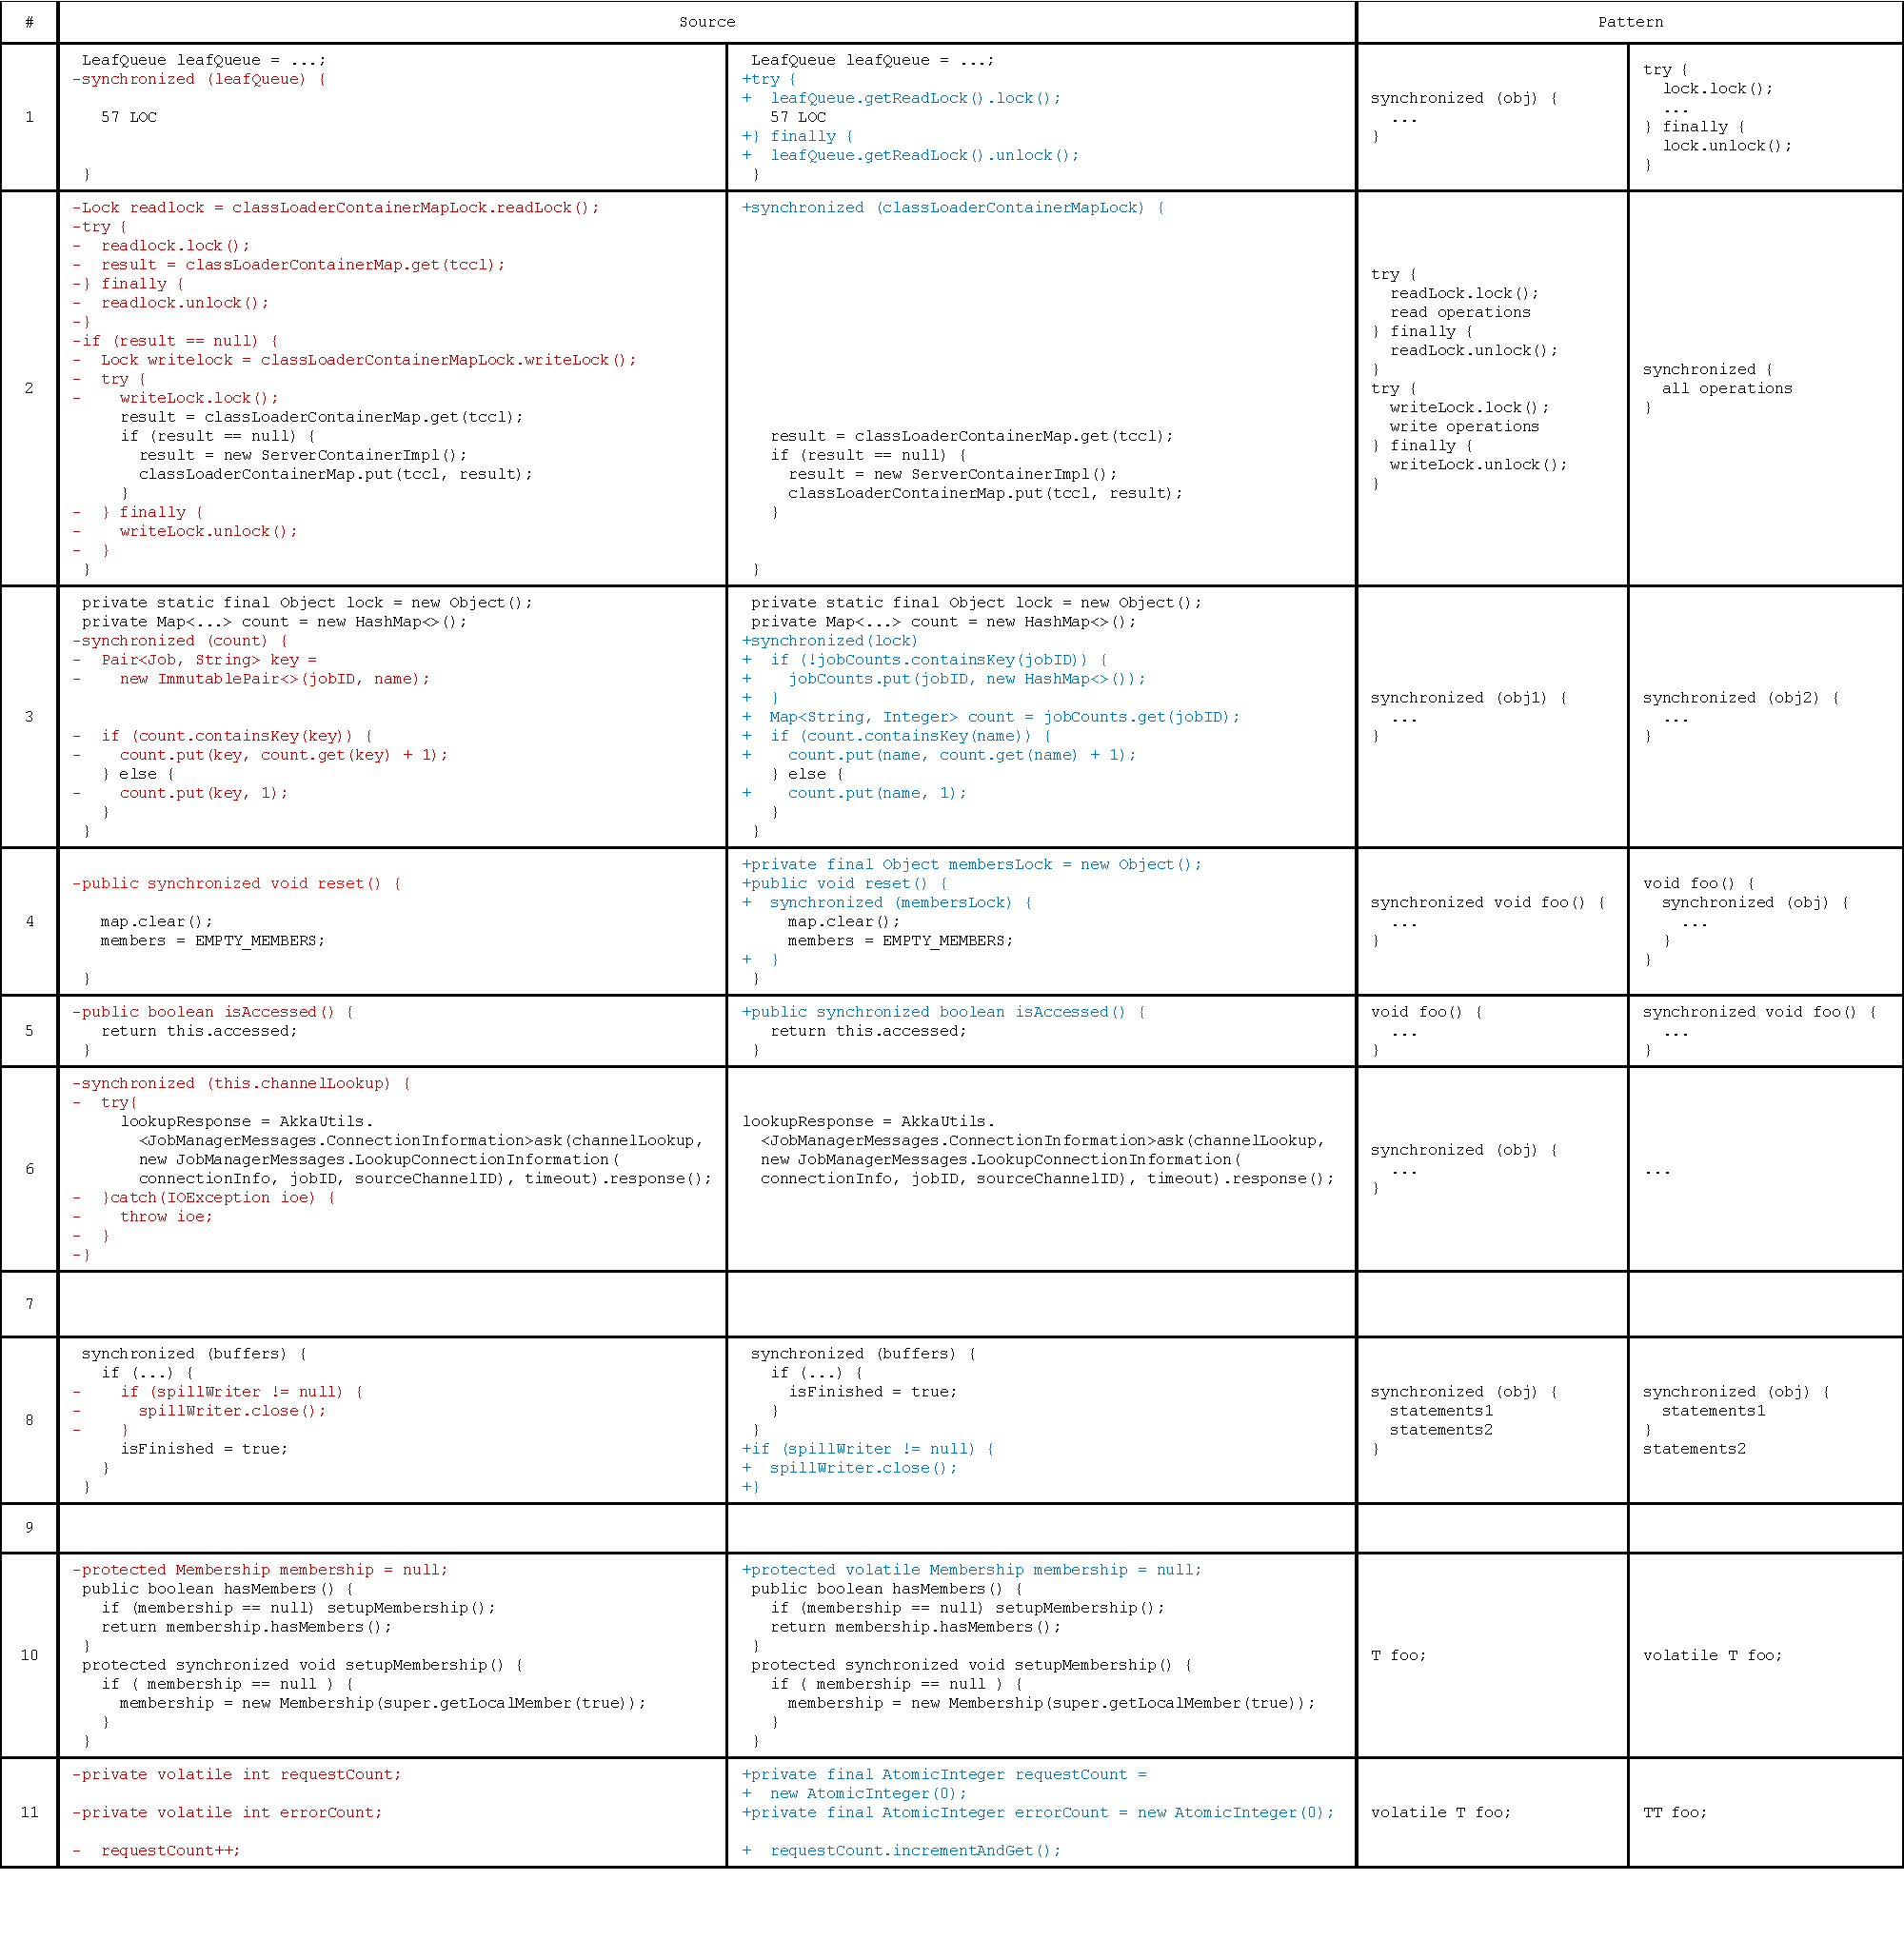
\includegraphics[width=1\textwidth]{patterns}
	\caption{Patterns}
\zhong{Please add labels to all your figures, tables, and sections. Please refer to your figures with labels. Please split the figure into two figures. Use Table instead of Figure. The font is too small.}
\end{figure*}

\noindent
\textbf{1. Changing lock types.} It is feasible to lock resources with different mechanisms. For example, Java has a keyword, \CodeIn{synchronized}. The keyword can lock a block of code lines. With the keyword, programmers do not have to acquire and release resources explicitly. Alternatively, programmers can explicitly lock resources with APIs (\emph{e.g.}, \zhong{add example}). \zhong{Please introduce the benefits of explicit locks.}

We can also view locks in a different perspective like exclusive and shared locks \cite{journals/jacm/KedemS83}. \zhong{Please explain what exclusive and shared locks are, and their benefits.}

%ReentrantLock, ReentrantReadWriteLock, StampedLock are all API level locks in Java. Although 'synchronized' keyword is convenient and straightforward, we need other locks when we have more requirements. ReentrantLock is a reentrant lock, which means a lock can be acquired repeatedly in the same thread. It is a exclusive lock with the similar behaviour as monitor lock but has more features such as fairness, condition and tryLock. ReadWriteLock is a pair of locks, which allows concurrent access to read operations when there is no write operation going on but exclusive access to write operations. StampedLock is a lock which provides three modes, namely writing, reading and optimistic reading. This lock is usually used in design of thread-safe classes.
Programmers can change their lock types due to various considerations. For example, the \CodeIn{synchronized} keyword can fail to satisfy fairness (\zhong{What is fairness? Why does it matter?}), programmers have to change such implicit locks to explicit locks. \zhong{Add an example for each situation.}

%fad9609d13e76e9e3a4e01c96f698bb60b03807e
%\begin{figure*}
%	\centering
%	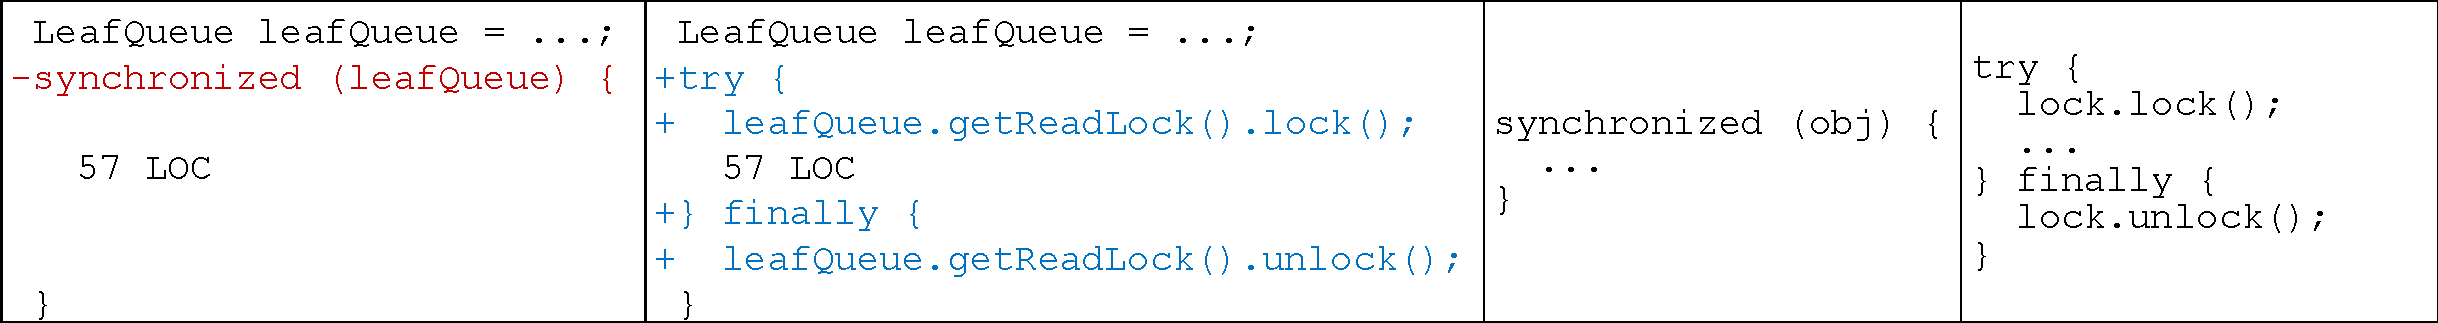
\includegraphics[scale=0.3]{locktype1}
%	\caption{Example 1}
%\end{figure*}

Example 1 is an example of YARN-5825\footnote{\url{https://issues.apache.org/jira/browse/YARN-5825} To save space, we remove the URLs of the other Apache issues. Their URLs can be built by replacing the above URL with their issue number. \zhong{Please remove the URLs}} - \texttt{ProportionalPreemptionalPolicy} could use \texttt{readLock} over \texttt{LeafQueue} instead of a synchronized block. It is a major bug of Hadoop project. They used a synchronized block to synchronize in various places, which can be replaced with a reader lock. \texttt{LeafQueue} is a method \texttt{getReadLock} which is inherited from its base class. This method returns an instance of \texttt{ReentrantReadWriteLock.ReadLock}. There are many different locks which can be used to synchronize. A reader lock is more lightweight than a synchronized block and it allows multiple threads to read simultaneously and hence improves performance under the scenario where most of the operations are reading.

%3e4b1ae6dc786b268505aa2e64067432519c2bcf
%\begin{figure*}
%	\centering
%	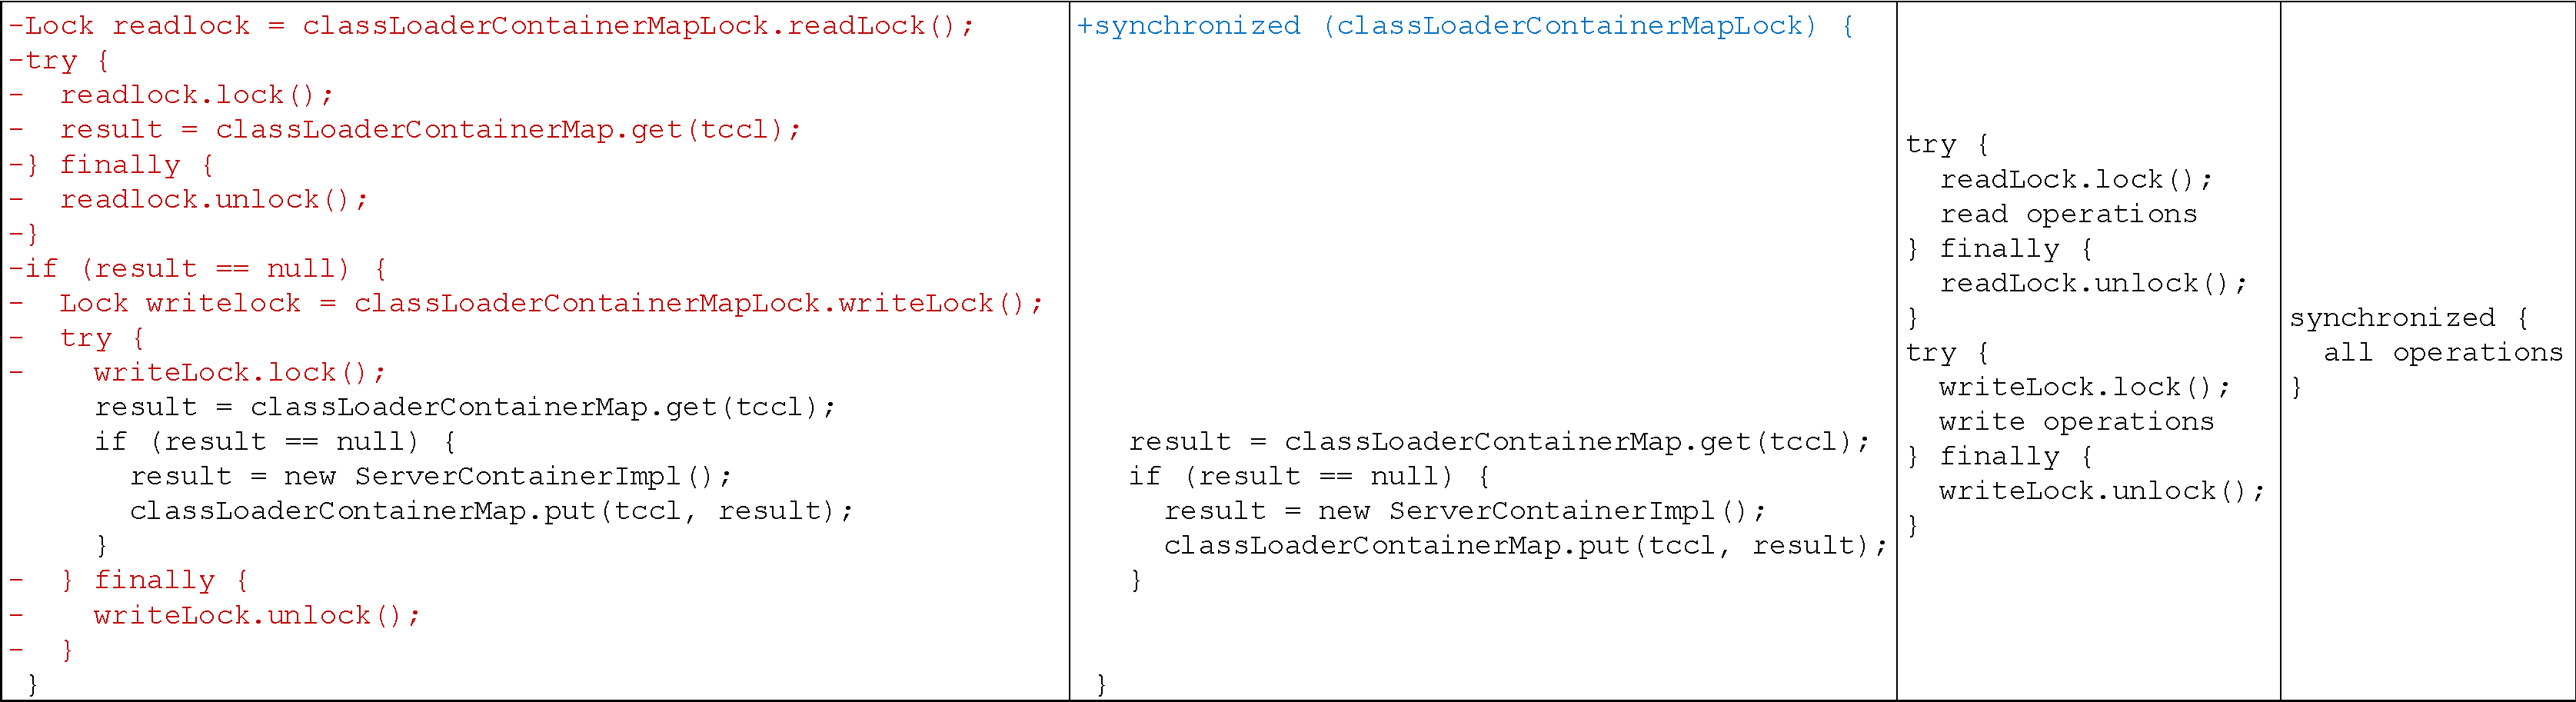
\includegraphics[scale=0.3]{locktype2}
%	\caption{Example 2}
%\zhong{It may be better, if you merge the example figures into a table like Table 1.}
%\end{figure*}



\zhong{Please replace all texttt with CodeIn.} 


They also might switch to a reader-writer lock \cite{journals/cacm/CouroisHP71} from a normal lock to improve concurrency when there are plenty of concurrent read operations. Here are some examples. \zhong{add an example for this.}

Example 2 is an example in Tomcat. \zhong{The issue number?} The developer said a \texttt{ReadWriteLock} cannot guard a \texttt{WeakHashMap}. It is because get() may modify the \texttt{WeakHashMap}, in which case a reader lock is not enough. A plain old lock or synchronization should be used. In this example, the synchronization is used finally. This example is more complex than the previous one although they seem a bit similar. %todo more detail


 When they find that they only need a simple exclusive lock, they switch to synchronized block. \zhong{add an example for this}


\zhong{Never use YOU in your paper!}
 
\noindent 
\textbf{2. Changing locked resources.} A program needs to lock a resource before it enters the corresponding critical section. Programmers can change locked resources, when they maintain concurrency code.  \zhong{Why they do that? To fix bugs?}
%\begin{figure*}
%	\centering
%	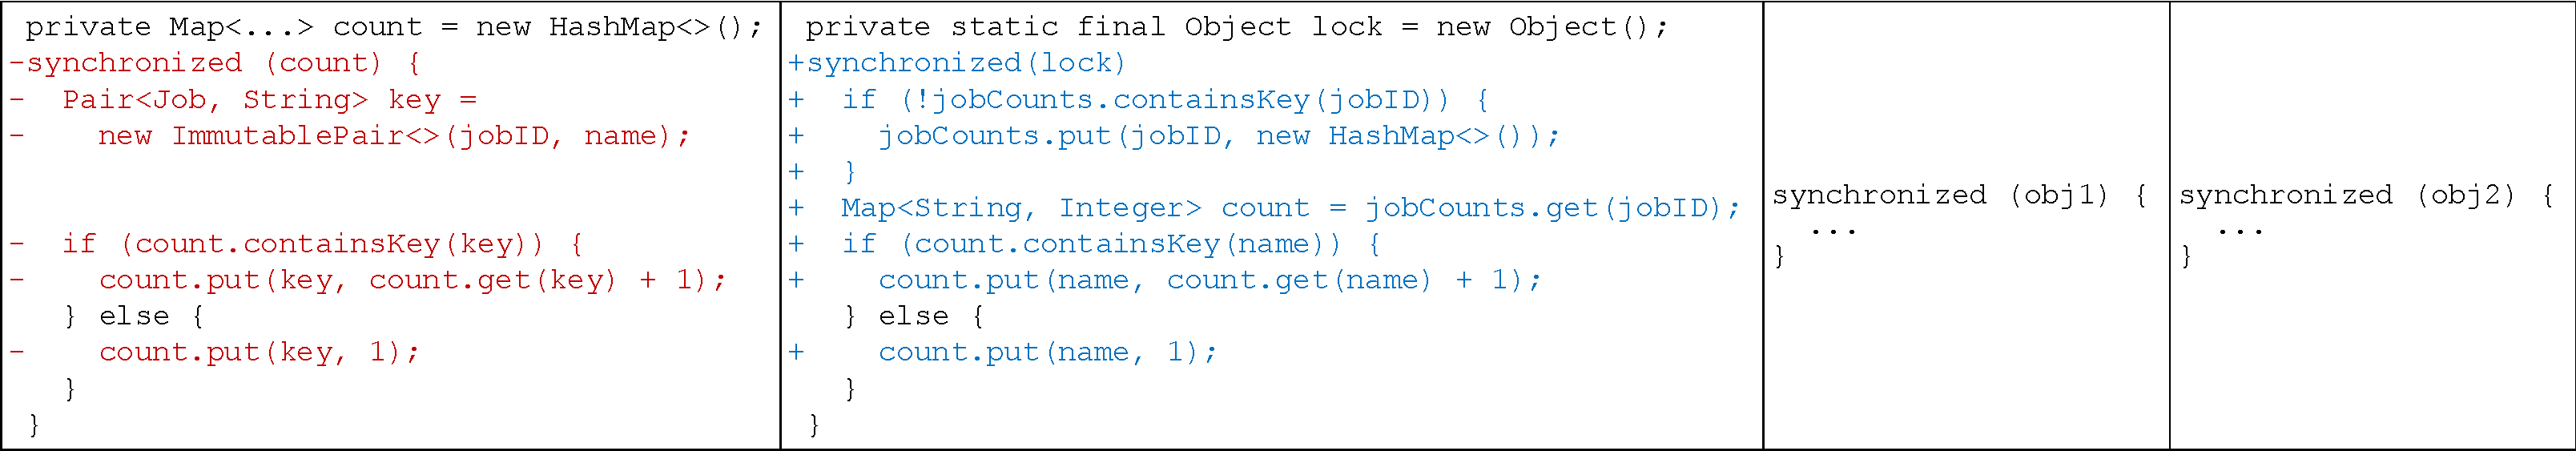
\includegraphics[scale=0.3]{lockins1}
%	\caption{Example 3}
%\end{figure*}

Example 3 is an example of FLINK-1419\footnote{\url{https://issues.apache.org/jira/browse/FLINK-1419}} - \texttt{DistributedCache} doesn't preserver files for subsequent operations, which is a major bug. The description said that it happens that the files are created yet for the operations when subsequent operations are going to access the same file in the \texttt{DistributedCache}. They synchronized on \texttt{count}, which is a map instance. Instead, they used \texttt{lock}, which is an instance of \texttt{Object} class. The difference is this instance is only used for synchronization while the former one has its own role not only as a lock. We do not need to blame preference of synchronization usage. This commit also made other changes about synchronization. They modified the critical sections as well.

%f0e627bb8c9daedb3b064027cac37ce4849bab64
\zhong{Explain a situation first, before you present its examples! After you present an example, further explain why the sample fit your situation!}

In example 4, The lock instance was originally the instance of the class and now is \texttt{membersLock}. They used single object (\texttt{membersLock}) for all locking as the commit message said. Using a separated locking instance can allow you to have more precise concurrency control than using synchronized methods.

\noindent
\textbf{3. Modifications on critical sections.} A critical section is a code block that is executed, when a thread locked the corresponding resources. \zhong{Based on what??}, we classify such modifications into three categories such as modifications on locks, statements, and locked resources. 


Modifications on locks either add or remove locks. For example, the ?? row in Table~\ref{} shows an example of adding synchronization. The method was not synchronized before. The basic reason of adding synchronization to existing code is the piece of code might be access concurrently. It is a change to fix a bug\footnote{\url{https://bz.apache.org/bugzilla/show\_bug.cgi?id=58386}}. This bug was reported by RV-Predict, a dynamic race detector. It said

\begin{lstlisting}
Reported by RV-Predict (a dynamic race detector) when running the test suite:
Data race on field org.apache.catalina.tribes.io.ObjectReader.accessed: {{{
Concurrent write in thread T93 (locks held: {Monitor@8a841fe, Monitor@8a9a01a})
\end{lstlisting}

When two or more threads access one object concurrently and at least one is modifying the object, a data race might happen. The easiest way to tackle this problem is adding synchronization to the access of the object.

%c93d9eaf363a535dff25cc4e7db400d879e73bb1
%Add option to use single actor system for local execution. Use local connection manager if a single task manager is used for local execution. Remove synchronized blcok in getReceiverList of ChannelManager which effectively serialized the connection lookup calls of a single task manager.
Modifications on statements change statements of critical sections. 
Example 6 shows an example of removing synchronization. Developers remove the synchronization of a code block. They said they used a single task manager and removed synchronized block in \texttt{ChannelManager}. If you find the code will not be accessed concurrently or it can be accessed safely in a concurrent way, you do not need to synchronize the code.

\begin{lstlisting}
commit 7e56bfe40589a1aa9b5ef20b342e421823cd0592
HDFS-4200. Reduce the size of synchronized sections in PacketResponder. Contributed by Suresh Srinivas.

-    synchronized void enqueue(final long seqno,
-        final boolean lastPacketInBlock, final long offsetInBlock) {
-      if (running) {
-        final Packet p = new Packet(seqno, lastPacketInBlock, offsetInBlock,
-            System.nanoTime());
-        if(LOG.isDebugEnabled()) {
-          LOG.debug(myString + ": enqueue " + p);
+    void enqueue(final long seqno, final boolean lastPacketInBlock,
+        final long offsetInBlock) {
+      final Packet p = new Packet(seqno, lastPacketInBlock, offsetInBlock,
+          System.nanoTime());
+      if(LOG.isDebugEnabled()) {
+        LOG.debug(myString + ": enqueue " + p);
+      }
+      synchronized(this) {
+        if (running) {
+          ackQueue.addLast(p);
+          notifyAll();
}
-        ackQueue.addLast(p);
-        notifyAll();
       }
     }
\end{lstlisting}

This is a commit of HDFS-4200\footnote{\url{https://issues.apache.org/jira/browse/HDFS-4200}} - Reduce the size of synchronized sections in \texttt{PacketResponder}, which is a major improvement. The previous two examples are very easy. This is a complex change compared to previous examples. This example contains multiple types of changes. They change the lock instance, remove synchronization of some code, add some new synchronized code. The developers said the size of synchronized sections can be reduced. It is always meaningful to remove the unnecessary synchronizations. Over-synchronization \cite{conf/sigsoft/GuJSZL15} is a real issue in real-world software.

%efca79cfb7b496b4bec70561cc94af069c644ef2
%[FLINK-2384] [runtime] Move blocking I/O call outside of synchronized block
%Problem: Waiting on asynchronous write requests with the partition lock can
%result in a deadlock, because all other operations on the same partition are
%blocked. It is possible that the I/O writer itself needs to access the
%partition, in which cases the whole program blocks.
%Solution: Move the wait outside the synchronized block. This was not necessary
%before, because no operation assumes the spilling to be finished when the
%finish call has returned.

\begin{figure}
	\centering
	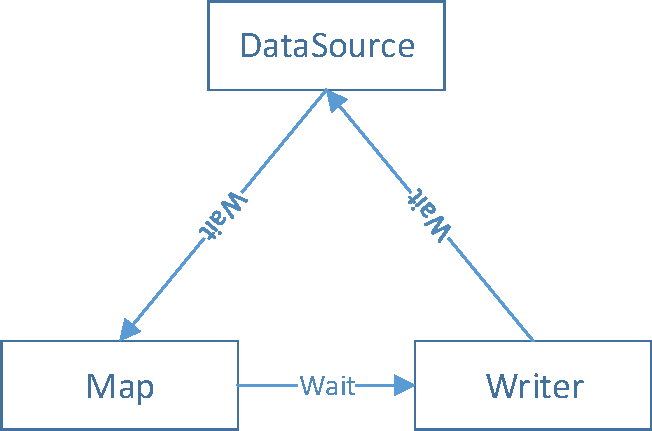
\includegraphics[height=1.7in]{deadlock}
	\caption{Deadlock}
\zhong{Please add resource columns and add edges to denote resource manipulations.}
\end{figure}


Modifications on locked resources change the criteria of entering critical sections.  \zhong{Please check whether the samples explain the corresponding situations.}

Example 8 is a fix of a bug. It is a critical bug issue\footnote{\url{https://issues.apache.org/jira/browse/FLINK-2384}} ``Deadlock during partition spilling''. A user reported the problem. Here is selected parts of the stack trace.

\begin{lstlisting}
"CHAIN DataSource (at createInput(ExecutionEnvironment.java:502) (org.apache.flink.api.java.hadoop.mapreduce.HadoopInputFormat)) -> FlatMap (FlatMap at readFlinkTuplesFromThriftParquet(ParquetThriftEntitons.java:96)) (7/8)" daemon prio=10 tid=0x00007f934005b000 nid=0x73c4 in Object.wait() [0x00007f93c16ac000]
java.lang.Thread.State: TIMED_WAITING (on object monitor)

"IOManager writer thread #1" daemon prio=10 tid=0x00007f93d8b7b000 nid=0x73a8 waiting for monitor entry [0x00007f93c2fc5000]
java.lang.Thread.State: BLOCKED (on object monitor)

"Map (Projection [0, 1, 2, 3, 4]) (7/8)" daemon prio=10 tid=0x00007f92b0434800 nid=0x74a3 waiting for monitor entry [0x00007f93a32f1000]
java.lang.Thread.State: BLOCKED (on object monitor)
\end{lstlisting}

The \texttt{DataSource} is waiting to be notified by the \texttt{Writer} when holding lock A. The \texttt{Writer} is trying to acquire lock B. But lock B is held by the \texttt{Map}. And the \texttt{Map} is trying to acquire lock A, which is held by the \texttt{DataSource}. Here is a waiting chain. This is a kind of bug known as deadlock. The problem is that the \texttt{DataSource} does not need to hold lock A while waiting to be notified. So the developer removed the unnecessary synchronization.

Example 9.

\noindent
\textbf{4. Changing the \CodeIn{volatile} keyword.} In Java, the \CodeIn{volatile} keyword denotes a variable that is saved in the main memory. For a \CodeIn{volatile} variable, a thread reads its latest value from the main memory, instead of the obsolete  value in the cache. Although it can improve the overall performance, races can occur, when multiple threads read and write \CodeIn{volatile} variables simultaneously.

%8313fa0f1ca277e9633a78f461804abc3c5515b8
%Fix https://bz.apache.org/bugzilla/show_bug.cgi?id=58392
%Double-checked locking needs to use volatile to be thread-safe

Example 10 is a fix of bug 58392\footnote{\url{https://bz.apache.org/bugzilla/show_bug.cgi?id=58392}} in Bugzilla. It is reported by a race detector that there is data race on field. Double-checked locking is a synchronization pattern in software engineering. It first check the condition without lock to reduce the time overhead when the condition is not satisfied. A typical usage of it is singleton pattern which uses lazy initialization to provide an unique instance during the process execution time in multi-threaded scenario. But sometimes programmers make some mistakes using this pattern like omitting \texttt{volatile} modifier of a class member. If \texttt{volatile} is not used, another thread which gets into the method may observe that \texttt{membership} has been assigned but the real initialization of the object has not been done yet due to the JVM's instructions reordering. Some work has been done in double-checked locking pattern \cite{conf/ispass/IshizakiDN14}, which can use this pattern automatically.

%560cd00890b3f6af2aca0c3a9d51a45f880692dd
%Fix a FindBugs warning (increment of volatile not atomic)

\zhong{Please explain why you need two samples for this situation.}

Example 11 shows that \texttt{volatile} is not almighty. The developer used FindBugs to check the code and it said increment of a \texttt{volatile} field is not atomic. This is a wrong demonstration of how to use \texttt{volatile}. The original code is not safe because increment is not an atomic operation. It includes read, calculate and write operations to complete the increment. So the developer used a thread-safe class instead.

\noindent
\textbf{5. Replacing self-written code with Parallel APIs.} Programmers can implement concurrency code by themselves, but later they realize that it is easier to call APIs that already implement their functionalities. For example, a previous version of Hadoop has the following code: \zhong{Replace the below commit with the buggy code.}

\begin{lstlisting}
commit a258263ecfa1d9efe03761f5e3b73e8e6ddb4a43
HDFS-4029. GenerationStamp should use an AtomicLong. Contributed by Eli Collins

-  private volatile long genstamp;
+  private AtomicLong genstamp = new AtomicLong();
...
-  public synchronized long nextStamp() {
-    this.genstamp++;
-    return this.genstamp;
+  public long nextStamp() {
+    return genstamp.incrementAndGet();
   }
\end{lstlisting}

Later, a programmer realizes that it is better to replace the above code with the \CodeIn{AtomicLong} class. He reported the issue (HDFS-4029), and set its priority as major. Here, \CodeIn{AtomicLong} is a thread-safe version of type long. It allows updating a \CodeIn{Long} value without explicit synchronization and it is fast. The fixed code is as follow:

\zhong{Replace the below commit with the fixed code.}

\begin{lstlisting}
commit a258263ecfa1d9efe03761f5e3b73e8e6ddb4a43
HDFS-4029. GenerationStamp should use an AtomicLong. Contributed by Eli Collins

-  private volatile long genstamp;
+  private AtomicLong genstamp = new AtomicLong();
...
-  public synchronized long nextStamp() {
-    this.genstamp++;
-    return this.genstamp;
+  public long nextStamp() {
+    return genstamp.incrementAndGet();
   }
\end{lstlisting}


\zhong{Rewrite the following sample as I did in the previous one.}

\begin{lstlisting}
commit 7f443f67eaa588323f912f3922cff9b699b38fbd
LUCENE-2779: Use ConcurrentHashMap in RAMDirectory

-  protected HashMap<String,RAMFile> fileMap = new HashMap<String,RAMFile>();
+  protected Map<String,RAMFile> fileMap = new ConcurrentHashMap<String,RAMFile>();
...
 @Override
 public final boolean fileExists(String name) {
     ensureOpen();
-    RAMFile file;
-    synchronized (this) {
-      file = fileMap.get(name);
-    }
-    return file != null;
+    return fileMap.containsKey(name);
 }
\end{lstlisting}

This commit is from lucene-solr. It is a commit for LUCENE-2779 which is a minor-priority improvement. It is better to use a thread-safe version collection ConcurrentHashMap instead of using HashMap and synchronizing the access code. This thread-safe class not only simplify the way of using a hash map, but also improve the performance compared to manual synchronization like the example because the implementation of ConcurrentHashMap is carefully designed. Retrieval operations do not acquire any locks at all and update operations do not lock the entire map. It supports full concurrency of retrievals and high expected concurrency for updates.

%\textbf{Other class replace}
%
%\textbf{Thread resource management}
%
%When we do concurrent programming, we need to pay attention to resource management such as threads, locks.
%
%Thread management is to deal with the management of thread-related resources.
%
%\textbf{Thread sleep wait notify}
%
%It is a another way of synchronization which is less common than locking.
%
%\textbf{Final in multiple threads}

\subsection{RQ2. The usefulness of our change patterns.}
\label{sec:result:sample}

\zhong{Try to add an example for each change pattern.}


 We have found some contexts which are suitable for the change patterns in different projects.

\begin{lstlisting}
+import java.util.concurrent.ThreadLocalRandom;
public class DRandom {
-    private static ThreadLocal<Random> random = new ThreadLocal<Random>() {
-        protected Random initialValue() {
-            return new Random();
-        }
-    };
public static Random get() {
-        return random.get();
+        ThreadLocalRandom.current();
}
}
\end{lstlisting}

This example shows a change from ThreadLocal$<$Random$>$ to ThreadLocalRandom from JDK7. It is from a Schmince-2, a game on Google Play. We make the change and our pull request\footnote{\url{https://github.com/derekmu/Schmince-2/pull/1}} has been accept. ThreadLocalRandom should be used when available in place of ThreadLocal$<$Random$>$. For JDK7 the difference is minimal, but JDK8 starts including optimizations for ThreadLocalRandom. The ThreadLocal class provides thread-local variables. The ThreadLocalRandom class is a random number generator isolated to the current thread.

\subsection{RQ3. What are the change trends of using parallel APIs}
\label{sec:result:trend}
\begin{table}
	\centering
	\caption{Top 10 Active Classes}
\label{table:topapi}
	\begin{tabular}{|c|c|}\hline
		Class&Occurrence\\\hline
		AtomicInteger&6,891\\
		AtomicBoolean&4,180\\
		ConcurrentHashMap&3,976\\
		AtomicLong&3,926\\
		CountDownLatch&3,211\\
		AtomicReference&2,254\\
		Executors&2,026\\
		ThreadPoolExecutor&1,617\\
		LinkedBlockingQueue&1,553\\
		ConcurrentLinkedQueue&1,435\\\hline
	\end{tabular}
\end{table}

%\begin{figure}
%	\centering
%	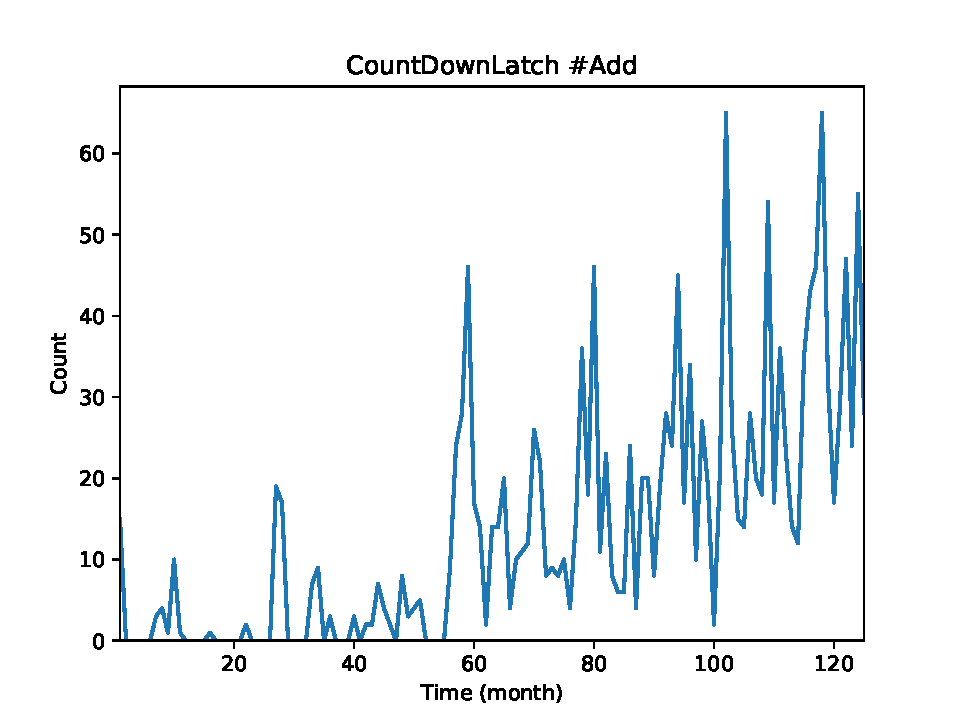
\includegraphics[height=1.5in]{CountDownLatchAdd}
%	\caption{Addition of CountDownLatch}
%\end{figure}
%
%\begin{figure}
%	\centering
%	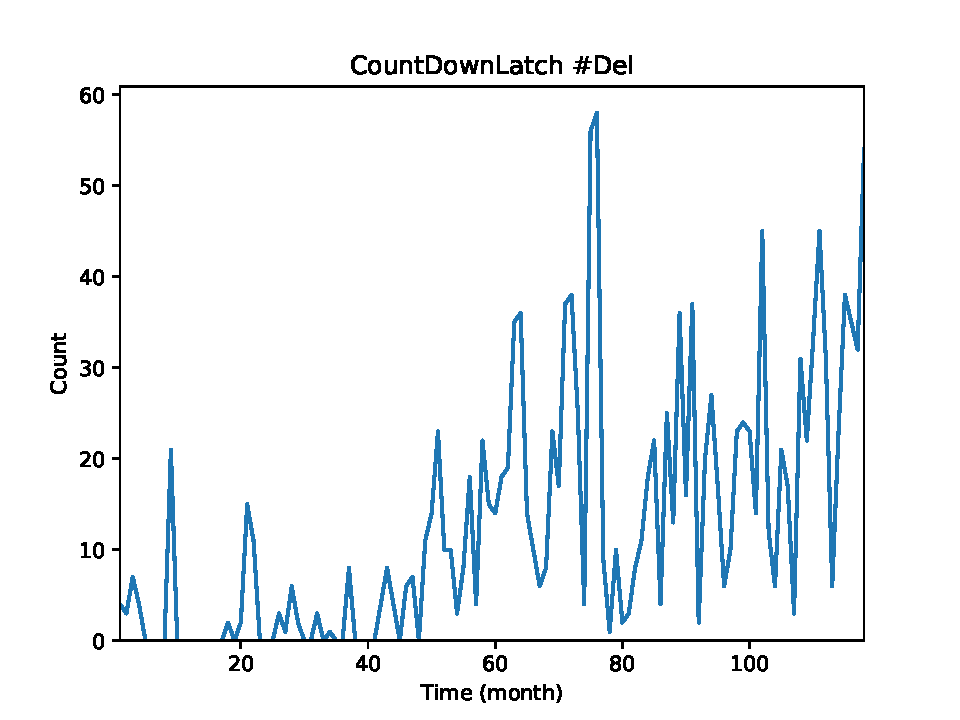
\includegraphics[height=1.5in]{CountDownLatchMinus}
%	\caption{Removal of CountDownLatch}
%\end{figure}

\begin{figure}
	\centering
	\subfigure[Ascending]{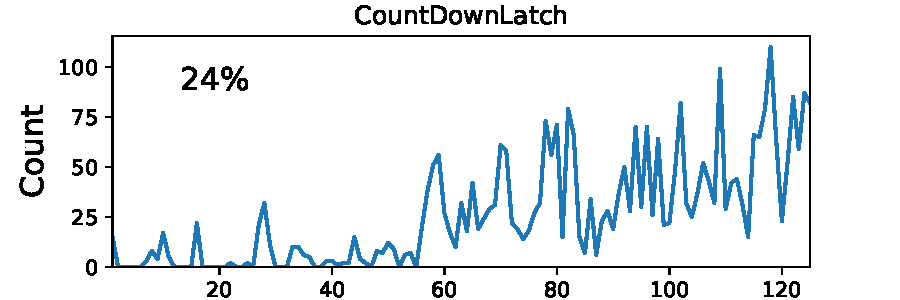
\includegraphics[height=0.8in]{CountDownLatch}}
	\subfigure[Descending]{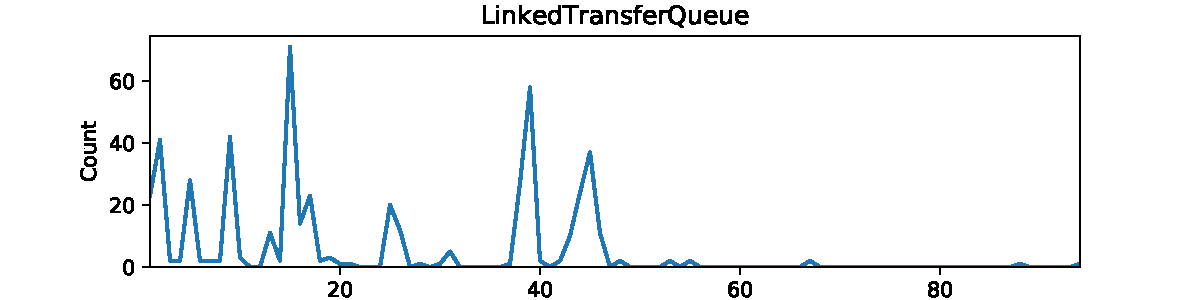
\includegraphics[height=0.8in]{LinkedTransferQueue}}
	\subfigure[Hybrid]{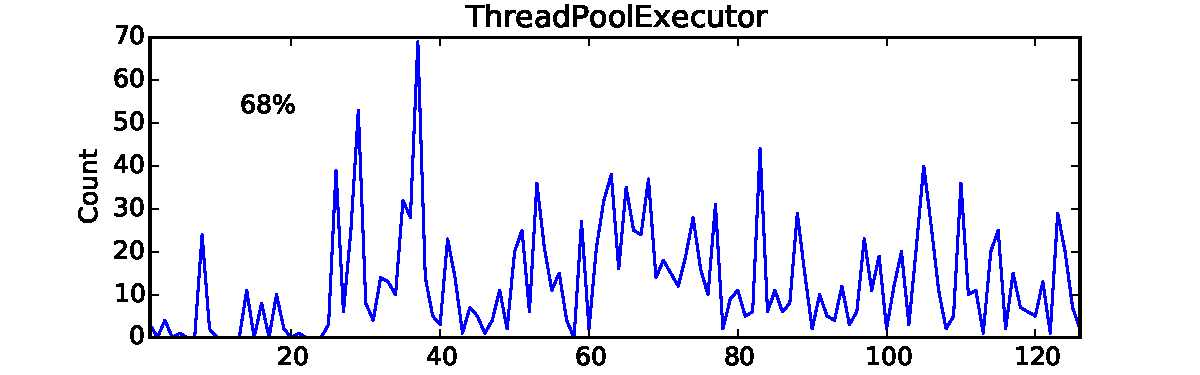
\includegraphics[height=0.8in]{ThreadPoolExecutor}}
	\caption{Typical Trend of Change Frequency}
\zhong{Please add more detailed figures! Divide them by their frequencies first! Add \%}
\end{figure}

Table~\ref{table:topapi} shows the top ten active parallel API classes. \zhong{Explain columns.} For example, the most common class in changes is \texttt{AtomicInteger}. There are 6,891 changes which are related to this class. This indicates that this class is very popular. We notice that the first several classes in the table are all famous and easy to use. The values of different classes vary. For the last 10 classes, the sum of their values is only 148. \%10 classes account for over 50\% occurrence of changes

We draw the tendency chart of each class as time goes. Figure 4 shows 3 typical tendencies of these charts. They are ascending lines, descending lines and hybrids. Figure (a) shows an example of ascending tendency. It is \texttt{CountDownLatch}. We are not meaning it is in a strict ascending order. Its overall tendency is rising. Figure (b) shows an example of descending tendency. It is \texttt{LinkedTransferQueue}. However, most charts are like figure (c). They are fluctuating without certain ascending or descending tendency. There are 13 ascending charts, 4 descending charts and 36 hybrid charts.

%We write a program to count and analyze concurrent programming classes usage. Table IV shows top 10 classes added and deleted in the history. Some classes are both active in the added and the deleted column like AtomicInteger and CountDownLatch. This is not surprising because a deletion of class does not mean this class is abandoned. This also indicates this class is active. An interesting observation is that deletions appear more than addition.

%We draw line for addition and removal of each class. Figure 3 and figure 4 show examples. We can see that both numbers of addition and removal increase as a whole as time passing by. This indicates that this class is attracting developers' attention.

\subsection{RQ4. The correlations between commits and concurrency commits.}

\begin{figure*}
	\centering
	\subfigure[Cassandra]{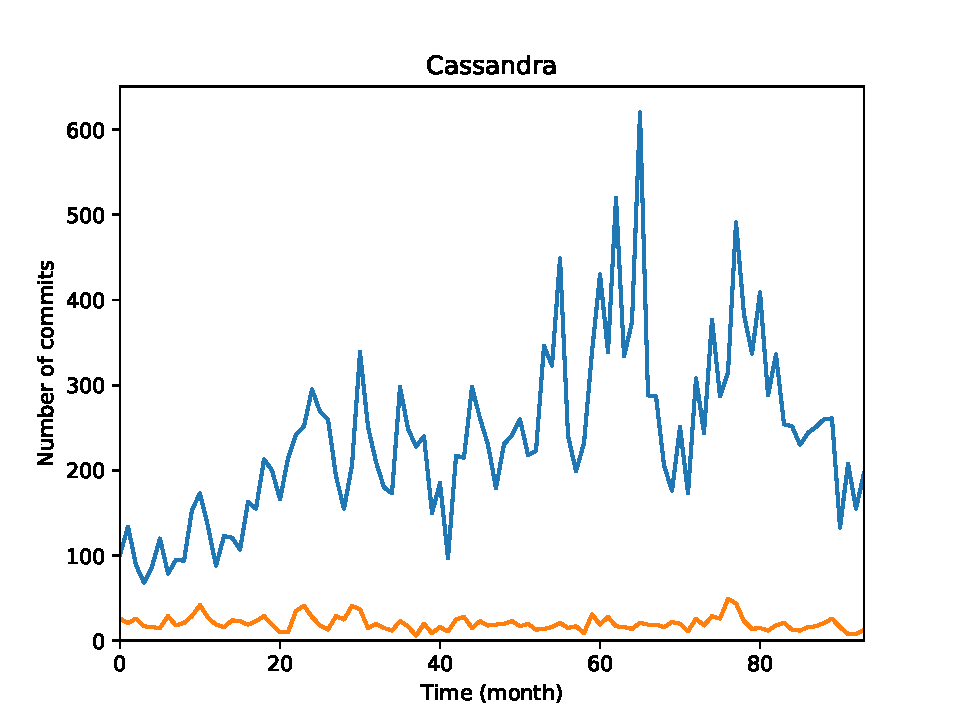
\includegraphics[height=1.2in]{cassandra}}
	\subfigure[Flink]{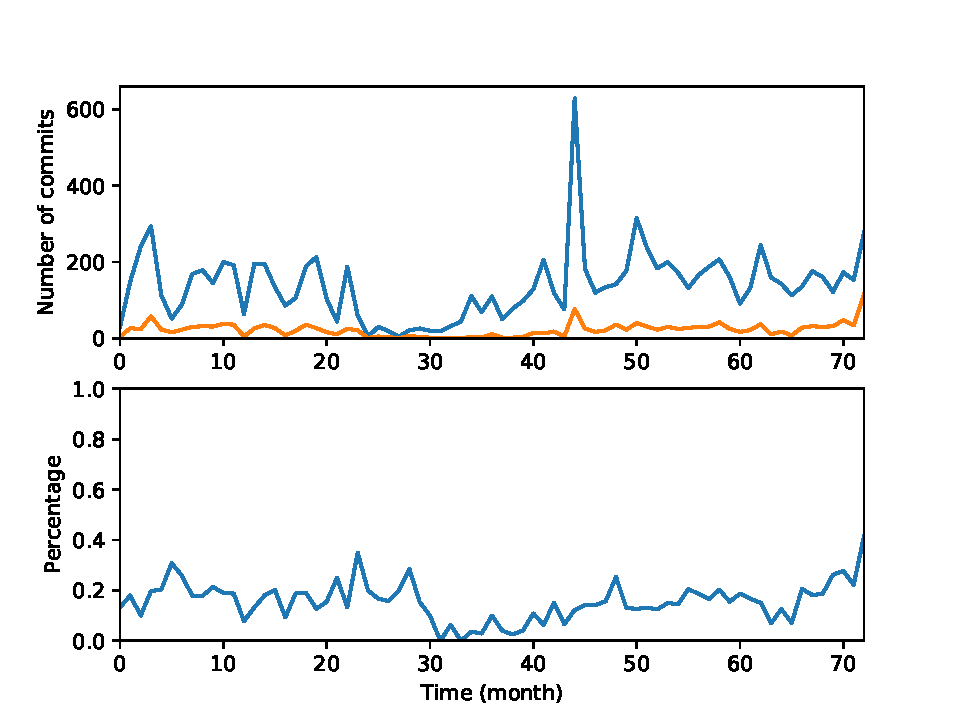
\includegraphics[height=1.2in]{flink}}
	\subfigure[Hadoop]{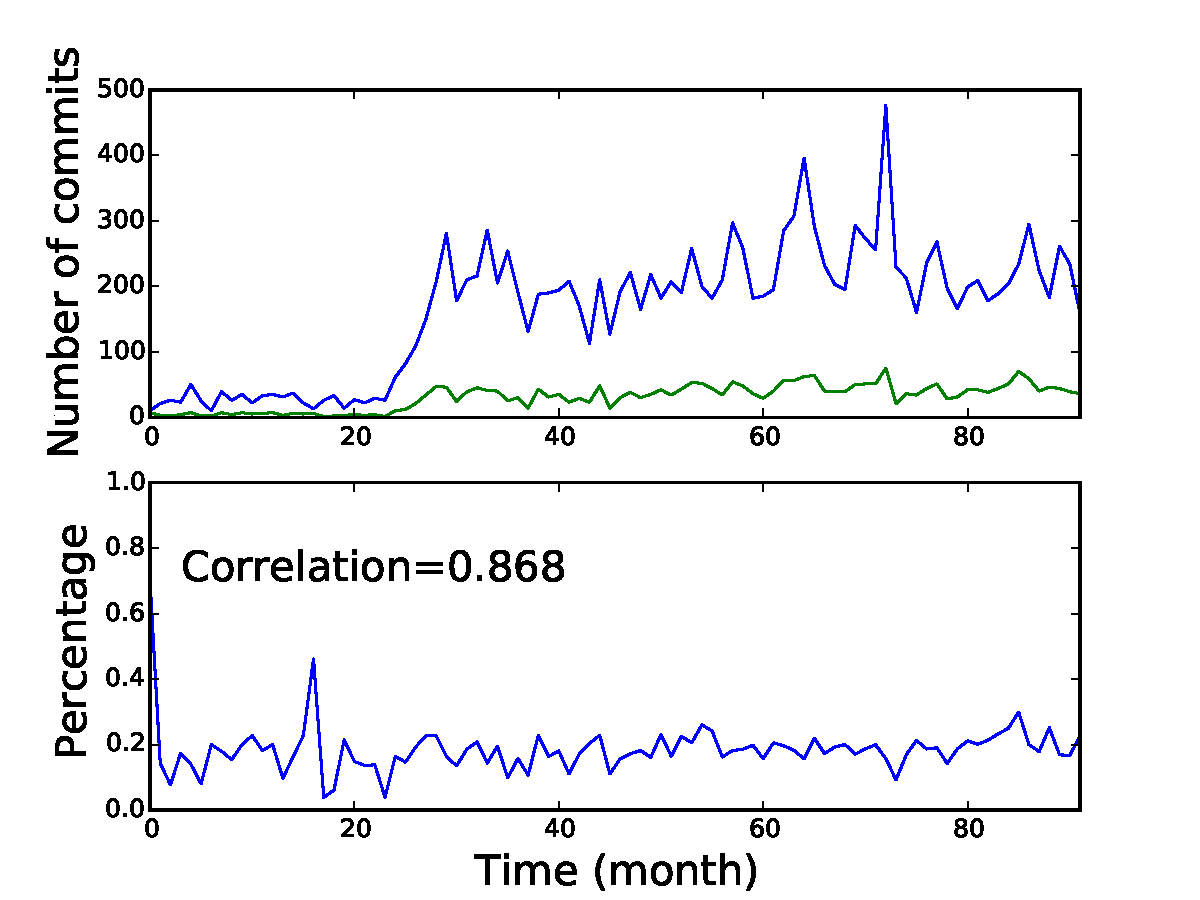
\includegraphics[height=1.2in]{hadoop}}
	\subfigure[Lucene-Solr]{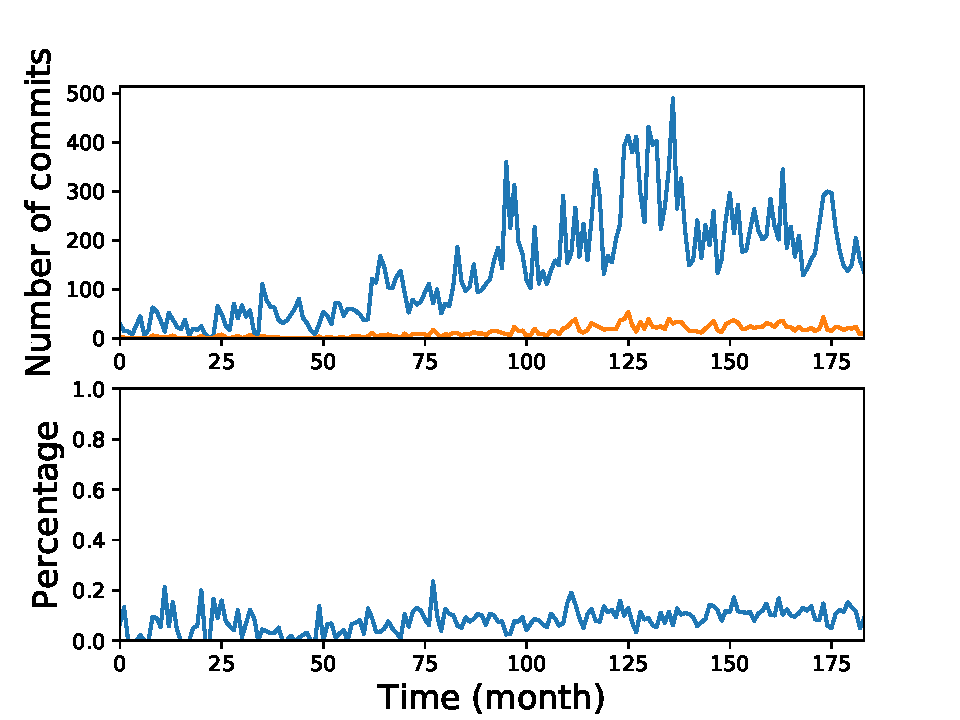
\includegraphics[height=1.2in]{lucene-solr}}
	\subfigure[Mahout]{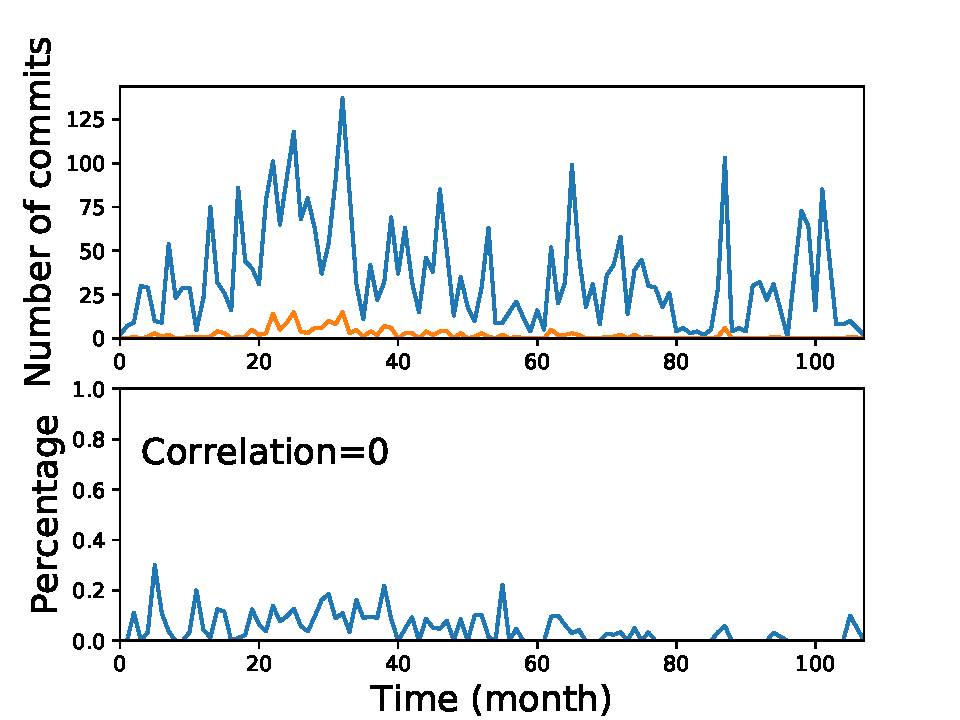
\includegraphics[height=1.2in]{mahout}}
	\subfigure[Netty]{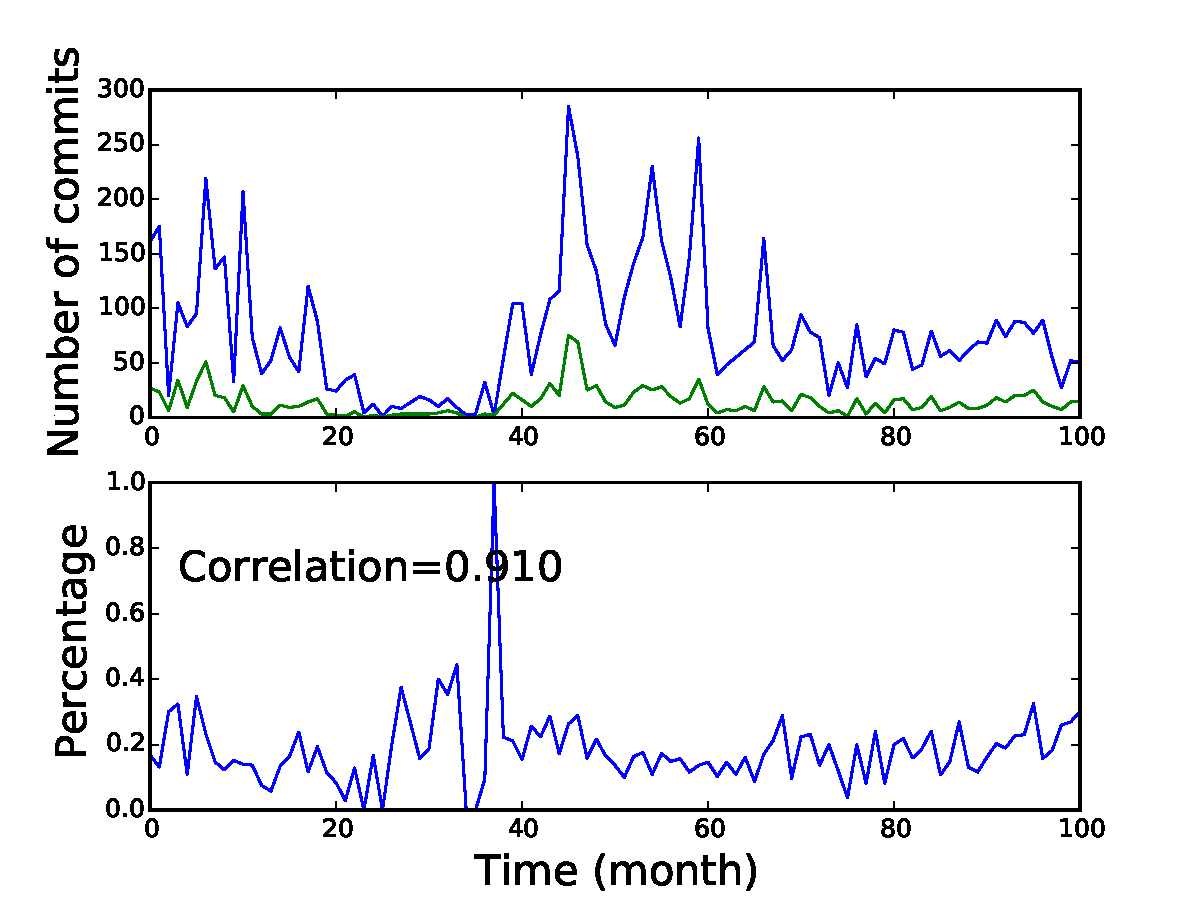
\includegraphics[height=1.2in]{netty}}
	\subfigure[Tomcat]{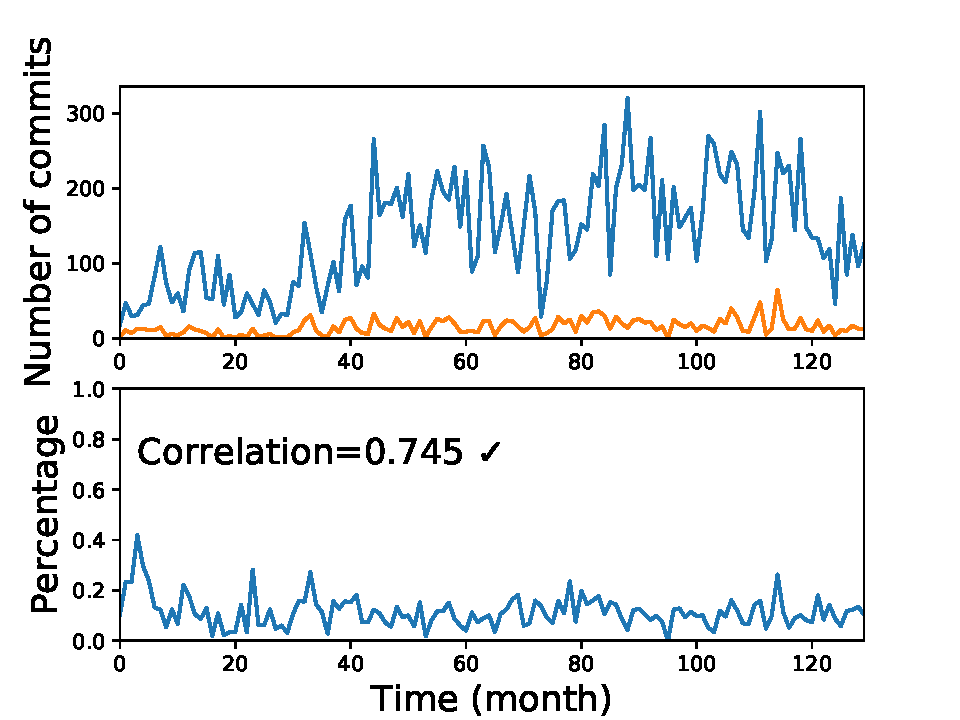
\includegraphics[height=1.2in]{tomcat}}
	\caption{Number of concurrent related commits compared to all commits}
\zhong{add confidence!}
\end{figure*}
\zhong{Cite and discuss Lu Shan's paper first, before you introduce your results. Explain why you conduct the study, given that Lu Shan already did that.}

Figure 1 shows the numbers of concurrent related commits and all commits of each month in all projects of our study. It also shows the percentage of concurrent related commits. Each subfigure has two subfigures inside. The x axis represents the time in month. The upper subfigure has two lines. The higher line shows the number of all commits while the lower line shows the number of concurrent related commits. The number of concurrent related commits is relatively small compared to the number of all commits. The two indexes have a positive correlation generally. The bottom subfigure shows the percentage of concurrent related commits. The percentages differ in project and time. For example, the percentage of concurrent related commits in mahout is relatively lower than other projects. The percentage in Hadoop is stable and high compared to other projects.
 
We calculate Spearman's rank correlation coefficient of number of commits and concurrency commits. Our result in a different language is similar to Gu's result. The coefficients are 0.094 for Cassandra, 0.844 for Flink, 0.868 for Hadoop, 0.896 for Lucene, 0.910 for Netty and 0.745 for Tomcat. Our result is consistent with Gu's result except one project.

\zhong{Explain whether your results are consistent with Shan Lu or not. }

\subsection{Threats to Validity}

The threats to internal validity include that our tool can omit some concurrency commits. Due to various issues, our tool can fail to identify all concurrency commits. To reduce the threat, we employ both the query-based search and a classifier in our study. The threat could be further reduced by more advanced identification techniques. The threads to internal validity also include obsolete commits. With the rapid development of software, such commits may present obsolete or even wrong usages. To reduce the threat, in our study, we prefer to recent commits. The threats to external validity include our selected projects and programming language. The number of the projects we select is small compared to the huge amount of open-source projects. The threat could be reduced by introducing more projects and languages in future work.

